\documentclass[11pt,a4paper,twocolumn]{article}
\usepackage{hyperref}
\usepackage[T1]{fontenc}
\usepackage[utf8]{inputenc}
\usepackage[left=0.5in,top=0.5in,right=0.5in,bottom=0.5in,nohead,nofoot]{geometry}
\usepackage{graphicx}
\usepackage{stfloats}
\usepackage[today,revrange,nofancy]{svninfo}
\svnInfo $Id: design_brief.tex 3034 2019-05-21 13:30:55Z cgat0038 $

\renewcommand\abstractname{Executive Summary}

\title{Design Brief: Group 1}
\author{
   Jonathan Cauchi,
   Cristina Gatt,
   Jerome Zerafa Gregory,
   Malcolm Vella Vidal 
}
\date{\svnMaxToday, Document v.\svnInfoMaxRevision}

\begin{document}

\maketitle

\abstract{
This document reviews the implementation and usage of a smart parking system. A system has been developed from scratch that allows clients to pass through a controlled and
tested barrier mechanism that allows for vehicle parking onto slots of which availability is regulated and exposed to the client via a system
that involves a microcontroller, multiple proximity sensors, a Liquid Colour Display (LCD) monitor and some LED's. In this document, possible problems regarding limited car parking
facilities and infrastructures have been addressed via a design analysis and implementation of a simple offline smart parking system from a limited time and resource point of view. 
The parking includes overall 2 entrance gates, 1 exit gate and 5 parking slots. Two proximity sensors have been assigned to each gate. The purpose of the first sensor is to detect
a metal object. Once detection occurs, the program will check for available parking slots. If available, the LED of that particular gate will glow green as to allow driver entrance. 
The second sensor is to verify that the driver is in the parking space and therefore the parking counter can be deducted accordingly. The same concept applies to the exit gate, except
that the second sensor of the exit gate is to verify that the client is outside the parking space, then the counter can be incremented. 
Once all parking slots are occupied, the program will ignore object detection from the sensors of the entrance gates until a slot is freed. The system makes sure to always allow driver 
exit and the count display of free parking slots via LCD monitor.
}

\section{Introduction}
In this assignment, a Parking System was implemented using the Embedded Artists LPC4088 board equipped with ARM Cortex M4. 

The aim of the System is to reduce the time spent finding parking spaces by Car Drivers. The System has two entrances and one exit. Each entrance and exit has an LED that lights up green when a car is detected in one of the entrances and there are empty parking spaces left in the Car Park. At the entrance points, there is an LCD Display that shows how many empty parking spaces are left. If the car park is full, cars will be able to get out of the parking but no cars will be able to get in as the LED does not turn green if there are no spaces left.

The remaining part of this Document is organized follows: Section 2 briefly describes the System Design together with a description of Hardware based on the requirements of the System. Section 3 describes the way the team implemented the project. Finally, Section 4 concludes the document with an overview of what was discussed in previous sections of the document. 

\section{System Design}

As can be seen in Figure \ref{fig:plot1}, the proposed system will have two entrances and one exit. The sensors are marked with an X on the diagram. 
 \begin{figure}
	\centering
	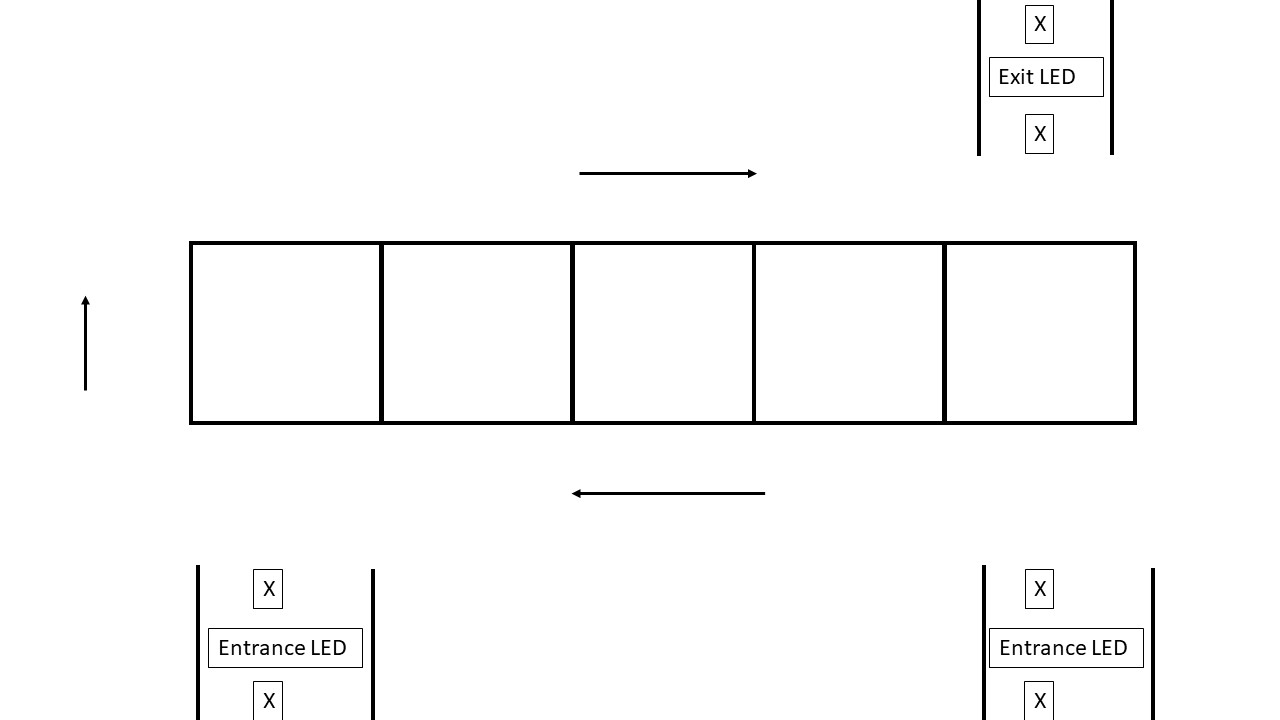
\includegraphics[width=85mm]{Car_Park}
	\caption{High-Level Design of the Car Park System Proposed.}
	\label{fig:plot1}
	\centering
\end{figure}

\subsection{Hardware}

\subsubsection{Input Hardware}

\begin{itemize}
\item The system makes use of Six Inductive Proximity Sensors. These sensors were bought online since the team could not find locally in stock. The sensors were bought via this link \url{https://www.aliexpress.com/item/32553311139.html}. They work at 5V. When connected with the microcontroller, they send a High Voltage, around 4.5V(equivalent Logic 1), when a metal is detected. When the sensor detects nothing, it return a very low voltage (equivalent to Logic 0).   

\end{itemize}

\subsubsection{Output Hardware}

\begin{itemize}
 \item The System makes use of a a Hitachi HD44780-based 2-line text LCD display. This comes included with the Embedded Artist board used for this assignment.
 \item The system also makes use of 3  RGB LEDs. These LEDs light Red or Green or Blue according to what voltage is sent through the respective wires. A logic 0 switches the RGB component off and a logic 1 switches it on. These were bought from a local vendor. 
\end{itemize}


These input/output hardware will be connected to, and implemented by, the ARM Cortex-M4 microcontroller, which will interact with the hardware and give it the instructions from the software. For it to work, the hardware and software aspects of the system must be cohesive and work together. For this problem to be handled the ARM ARMCM is used as it is:
\begin{itemize}
	
	\item 	Simple, easy-to-use programmers model
	\item 	Highly efficient ultra-low power operation
	\item	Excellent code density
	\item 	Deterministic, high-performance interrupt handling
	\item	Upward compatible with the rest of the Cortex-M processor family
\end{itemize}

\subsubsection{Connecting the Hardware with the MicroController}

\begin{figure}
	\centering
	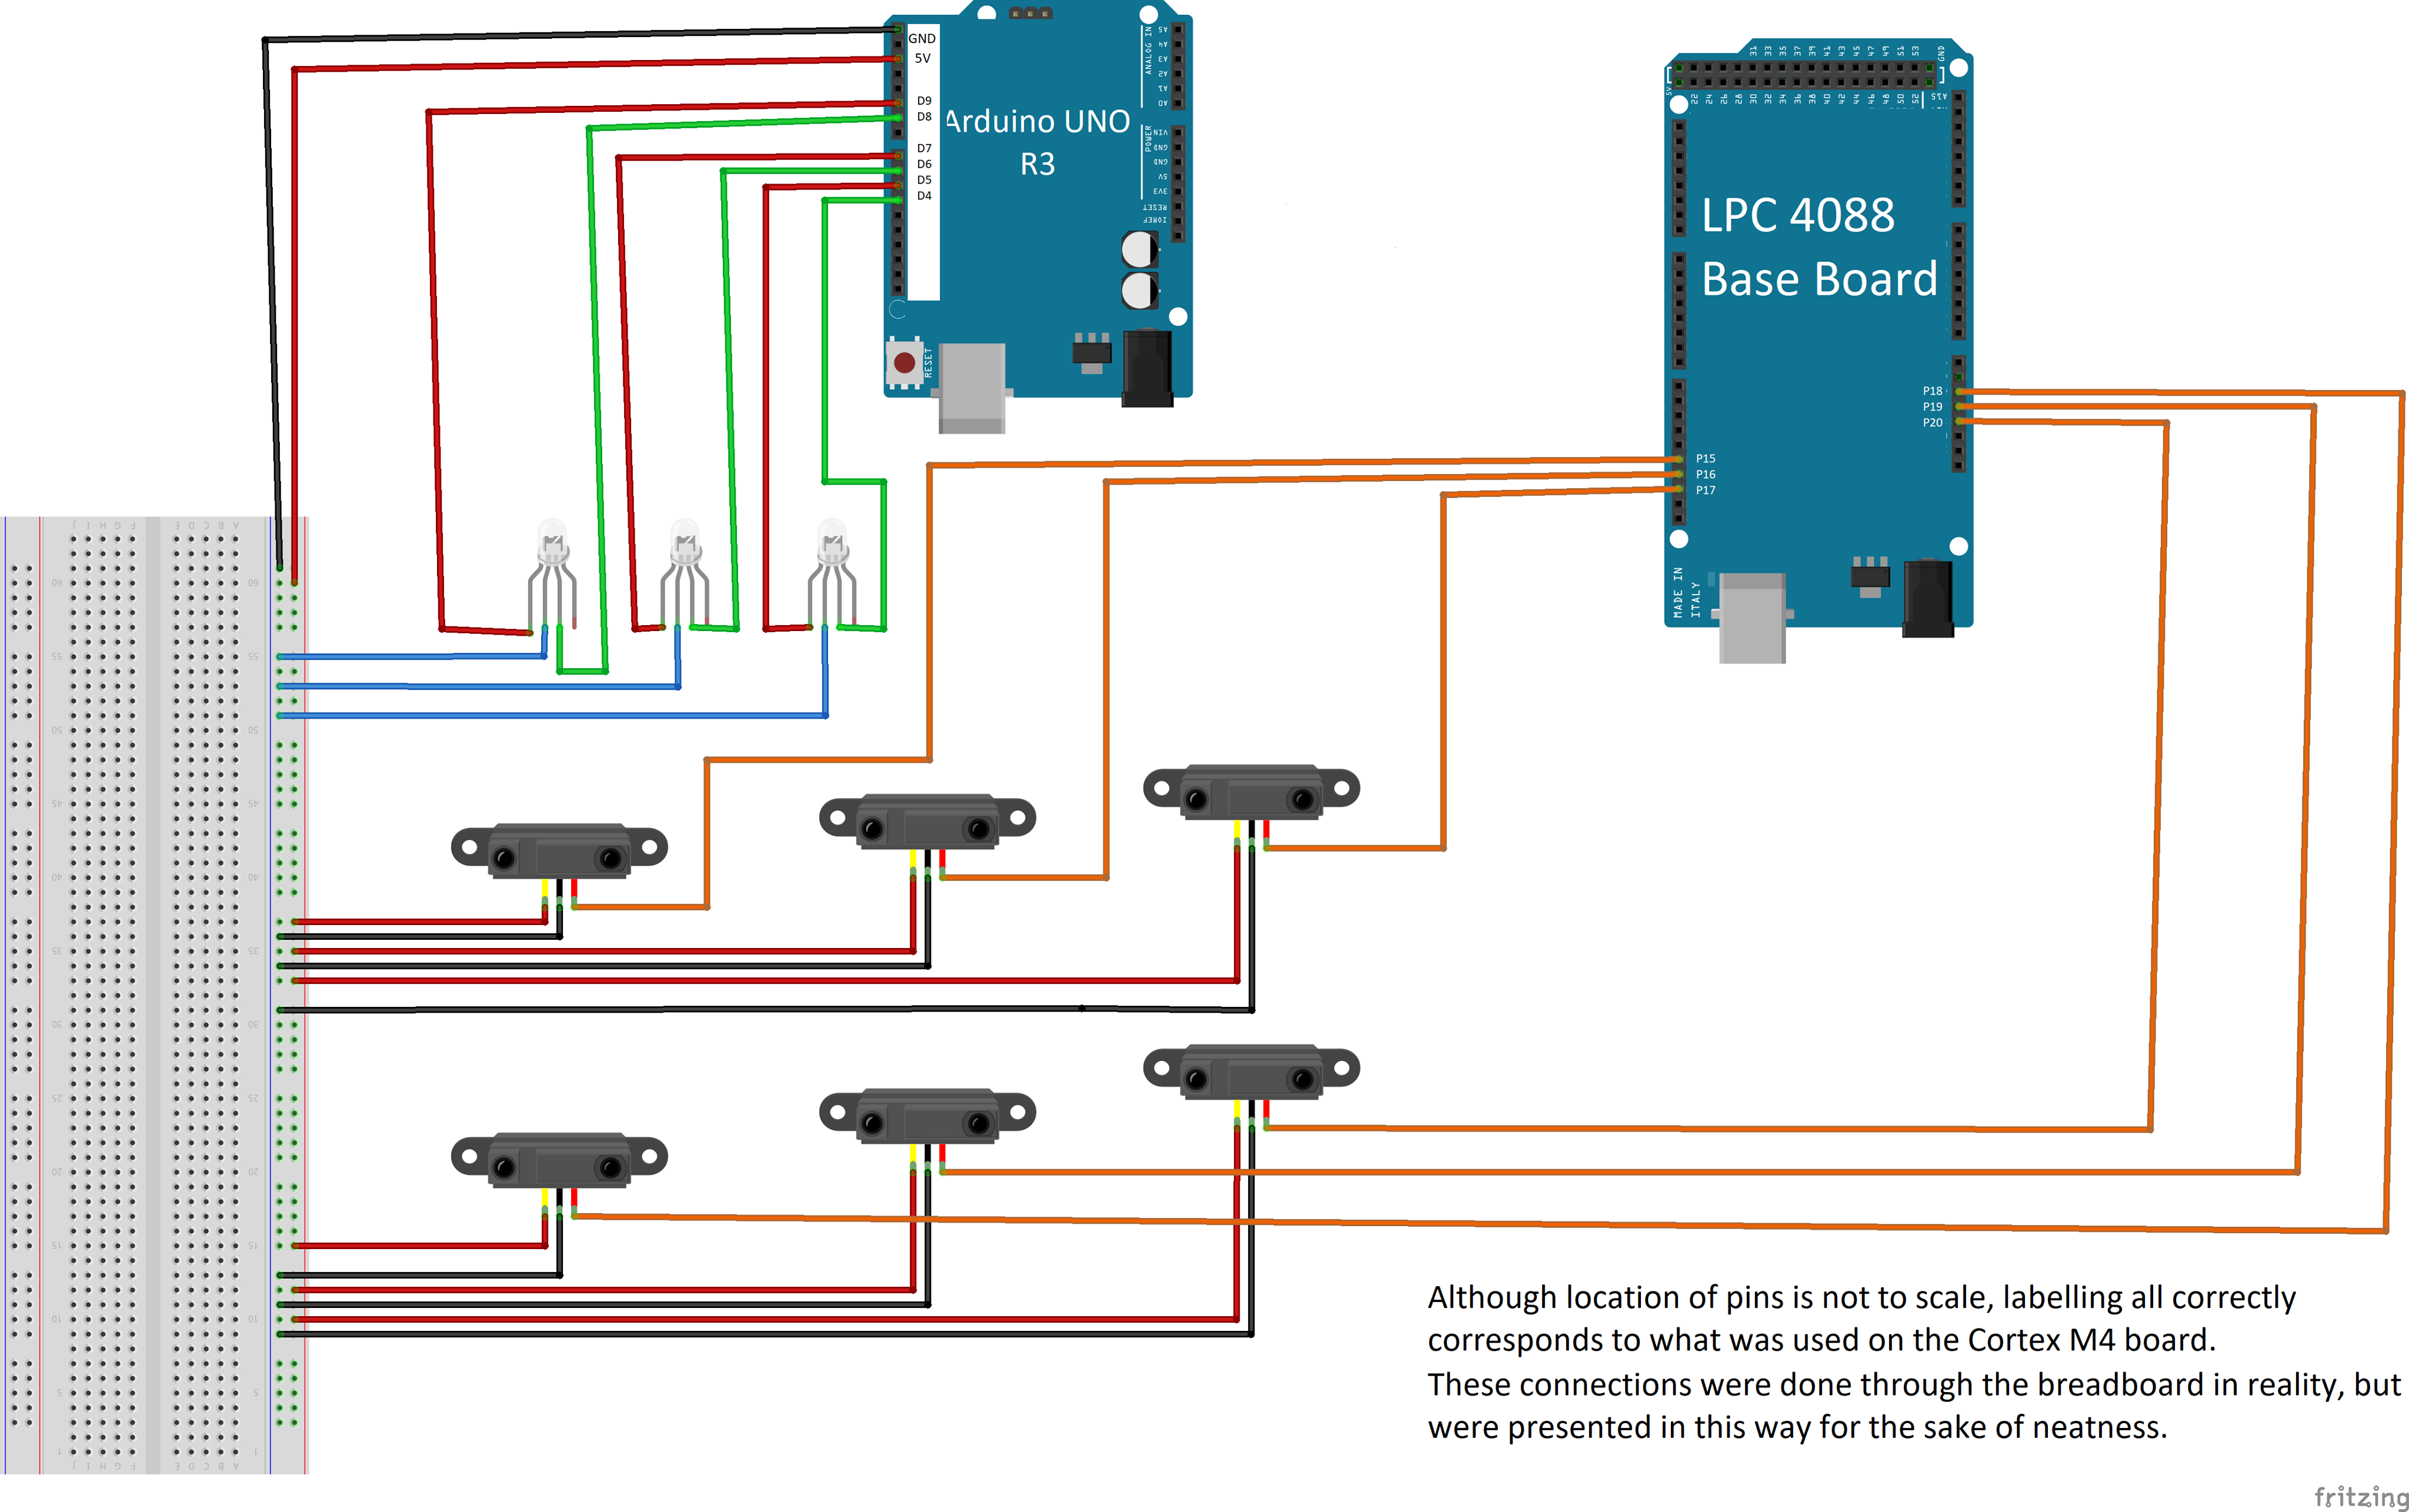
\includegraphics[width=85mm]{board}
	\caption{The way pins were connected with the board}
	\label{fig:Pins}
	\centering
\end{figure}
As the system contains of a lot of hardware components, a breadboard was used to connect all the components together. In Figure \ref{fig:Pins}, the way the components were integrated together. 

The pins used in the system are as follows (The pin in the second column signifies the reference of the Pin on the board while the pin in the third column signifies the Pin used in coding):


	
	\begin{table}
		\centering
	\begin{tabular}{ c c c }
		Pre-Entrance & P20 & P1\_31 \\ 
		Post-Entrance & P19 & P1\_30 \\  
		Red LED & P32 & P5\_2\\
		Gree LED &P34 & P0\_4    
	\end{tabular}
	\caption{Pins used for Entrance 1}
	\label{tab:2}
	\end{table}
	
	\begin{table}
		\centering
	\begin{tabular}{ c c c }
	Pre-Entrance & P18 & P0\_26 \\ 
	Post-Entrance & P17 & P0\_25 \\  
	Red LED & P39 & P5\_0\\
	Gree LED &P38 & P5\_1  
	 \end{tabular}
 		\caption{Pins used for Entrance 2}
 		\label{tab:3}
    \end{table}

	\begin{table}
		\centering
	\begin{tabular}{ c c c }
    Pre-Exit & P16 & P0\_5 \\ 
    Post-Exit & P33 & P0\_24 \\  
    Red LED & P37 & P5\_4\\
    Gree LED &P31 & P5\_3   
	\end{tabular}
	\caption{Pins used for Exit}
	\label{tab:4}
    \end{table}


\begin{itemize}
	\item Entrance 1: See Table \ref{tab:2}
	\item Entrance 2: See Table \ref{tab:3}
	\item Exit 3: See Table \ref{tab:4}
\end{itemize}

For the sensors, it is required to define the pins that are connected to the entrance and exit
sensors and which sensors should be connected to the servo motor and which sensors are not, if any are independent. A counter consisting of an integer value
is also required to be defined according to the available parking spaces/slots of which value will deducted and incremented according to the input registered.


\subsection{Dependencies}
\begin{itemize}
\item  The LED changes to green upon the pre-entrance/pre-exit sensor registering an input if and only if the parking is not full. 
\item The LED changes back to red upon either the post-entrance/post-exit sensor registering an input or when the system detects no input after the delay period has elapsed.
\item The  LCD Display changes only upon the system registering an input from the post-entrance/post-exit sensor. 
\end{itemize}

\subsection{Software}
Although in the original plan, the team planned to use C++, upon implementation, it was realized that C suited the needs of the project. Therefore, the solution was implemented using C. As an IDE, Keil UVision5 was used as recommended by the lecturer. 

Upon starting the implementation, it was noticed that a simple if-condition was not going to work for our project. Therefore, upon consulting with the lecturer, it was decided that States should be used to control the system execution. 
\begin{figure}
	\centering
	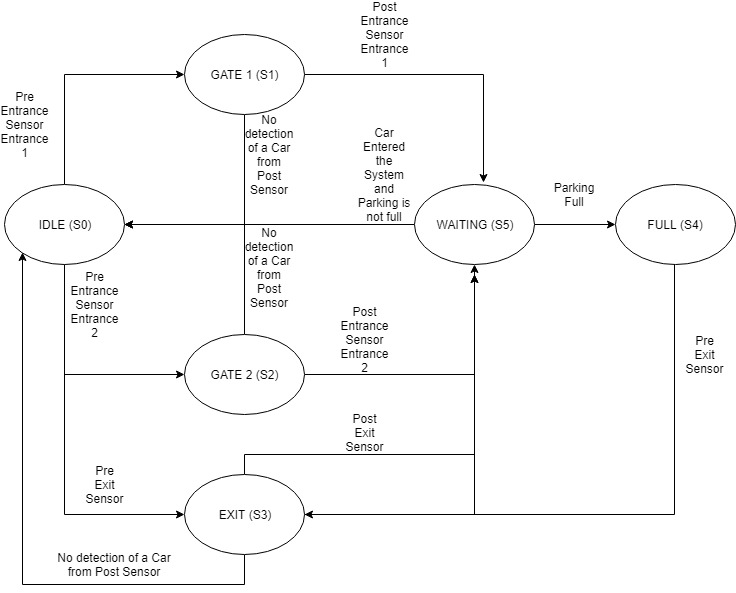
\includegraphics[width=85mm]{states}
	\caption{State Diagram for the System States.}
	\label{fig:states}
	\centering
\end{figure}
In Figure \ref{fig:states}, the States used by the System can be seen. The System is IDLE when no sensor is High and there are empty parking spaces. Upon starting the program, the system also enters the IDLE state. 

Upon the detection of a Pre-Entrance Sensor being High in Entrance 1 or 2, the System goes to state GATE 1 or GATE 2. It waits for a trigger from the Post-Entrance Sensor and if it receives nothing, it returns back to state IDLE. If it receives a High from the Post-Entrance Sensor, the System goes to state WAITING were it performs the necessary computations. Upon success, if there are no parking spaces left,the system goes to state FULL and if there are spaces left, it goes back to state IDLE. 

Upon detection of High Voltage from the Pre-Exit Sensor, the system goes to state EXIT and it waits again for a trigger from the Post-Exit Sensor. If it receives nothing, it goes back to the original state- either IDLE or FULL. If it receive a High Voltage from the Post-Exit Sensor, it performs the necessary computation and goes back to state IDLE. 

\begin{figure*}[b]
	\centering
	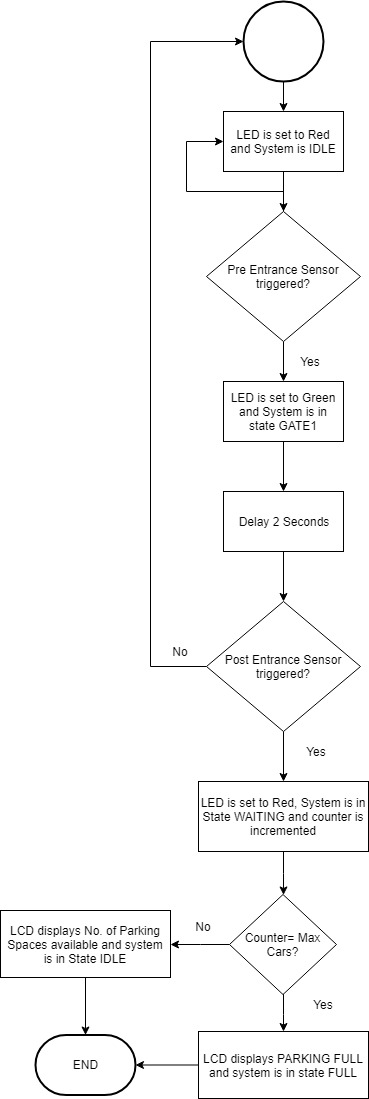
\includegraphics[width=85mm]{FlowChartEntrance}
	\caption{Flow Chart depicting the Entrance}
	\label{fig:entrance}
	\centering
\end{figure*}

\begin{figure*}[b]
	\centering
	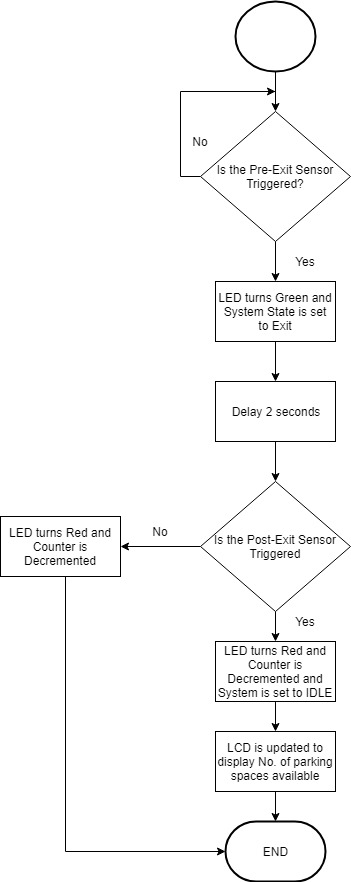
\includegraphics[width=85mm]{FlowChartExit}
	\caption{Flow Chart depicting the Exit.}
	\label{fig:exit}
	\centering
\end{figure*}
The main flow of execution is put in a While Loop to ensure continuous program execution. As described above, the system ensures that it is not locked up in a State from which it can not get out.This can be clearly seen in Figure \ref{fig:entrance} and \ref{fig:exit} which depicts the flow of the system using a flow chart. 


Several source files were needed to make it possible to interface with the hardware. The source files used were:

\begin{itemize}
	\item \verb|gpio.h\.c|: In this source file, the necessary functions to interface with the pins is found. The functions used were \verb|gpio_set_state| which sets the state of the Pin to whether it is output or input, \verb|gpio_set| which sets the value of a Pin to a logical 1 or 0 and \verb|gpio_get| which gets the logical value of a Pin.
	
	\item \verb|sensor.h\.c|: In this source file, function to interface with the sensors. The two available functions are \verb|sensor_get| which gets the logical value of a Pin and \verb|sensor_init| which sets the state of the pins used to interface with the sensors to Input. 
	
	\item \verb|lcd.h/.c|: In this source file, provided by the lecturer, several tweaks were made so that the LCD can display numbers. The four functions used were \verb|lcd_init|, \verb|lcd_print|, \verb|lcd_print_digit| and \verb|lcd_clear|.
	
	\item \verb|led.h/.c|: In this source file, also provided by the lecturer, the \verb|led_init| function was the only function used and it was edited to initiate the pins used for the LEDS as Outputs. 
\end{itemize}

\subsection{Problems encountered}

In the initial design brief, the team planned to use Servo Motors on entrance and exit of a car in the Parking. Unfortunately, after several attempts, it was decided that the team should use LEDs instead. In depth research was done about the Servo Motor and it was found that most of the times, this works by using the PWM. None of the team members have ever used this, and several attempts were made but these returned negative. Therefore, because time was pressing, it was decided that servo motors should not be used as it better to focus on other tasks at hand.
 
Another problem the team encountered was that one of the pins found on the board did not work and until we managed to find the problem, the system was behaving in unpredictable ways. This problem was solved by using another pin instead of the defective one. This is why in our project, we also make use of Arduino pins found on the LPC4088 board. 
\subsection{Testing the system}

Every line of code was tested before the components were integrated in the artifact. 

A few of the tests are:

\begin{itemize}
	\item A car entering from Entrance 1 and triggering the Post-Entrance sensor.
	\item A car entering from Entrance 2 and triggering the Post-Entrance Sensor.
	\item A car entering from an Entrance and does not trigger the Post-Entrance Sensor. 
	\item Two cars entering from different gates at the same time.
	\item A car exiting and not triggering the post-exit sensor.
	\item A car exiting and triggering the post-exit sensor.
	\item A car trying to enter when the car park is full.

\end{itemize}

All these tests passed. The team is aware that other tests might have been done to test that the system is robust. 

\subsection{Requirements}
	\begin{table*}[t]
		\centering
	\begin{tabular}{ c c  }
	REQUIREMENT & DESIGN  \\ 
	Real Time  & LED changes colour on Sensor Trigger  \\  
	One Digital Input & Inductive Proximity Sensor\\
	One Digital Output & LEDs\\
	One External Peripheral & LCD\\
	Error Indication & Displayed on LCD\\
	Multi-Threading & Multiple Entrances
\end{tabular}
\caption{Table of Requirements}
\label{tab:1}
\end{table*}

 Table \ref{tab:1} shows how our system meets the design specifications found in the Handbook.

\section{Management}
The management of the group was discussed thoroughly in the first and second group meetings. This was deemed important as we believed a solid foundation will be pivotal for the project completion going forwards. 
Primarily, an agile development approach was decided upon, which entails that the project will be split into pre-determined segments which are to be completed in sprints. Weekly meetings were set to Wednesdays from 12:00 to 14:00, and other slots in which the group will be all available were discussed just in case they were needed. Every week, the group split the workload into several tasks, set to each member to be completed until the next meeting.

During the Duration of the project, tasks were divided accordingly:
	
\begin{itemize}
	\item Research about components to be used and the aquiring of the components: Malcolm Vella Vidal and Jerome Zerafa Gregory
	\item The connection of components with the board: Malcolm Vella Vidal and Jerome Zerafa Gregory.
	\item Creating and mantaining the Backbone of the Project: Cristina Gatt
	\item Servo Motor Research, LEDs implementation, LCD implementation: Jonathan Cauchi. 
	\item Artifact: All the team members
	\item Minutes and Agendas: A different team member every week.
\end{itemize}

\begin{figure*}
	\centering
	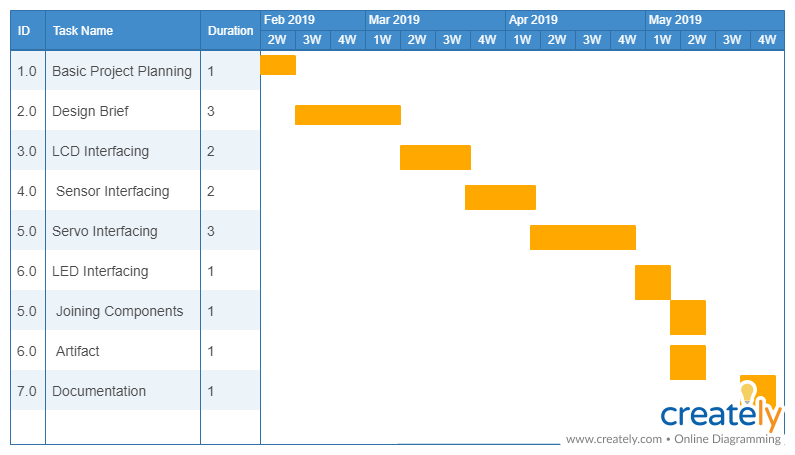
\includegraphics[width=\textwidth]{gantt}
	\caption{Gantt Chart of how the problem was tackled}
	\label{fig:gantt}
	\centering
\end{figure*}

Despite this task division, it was stressed that the group is well informed on what is going on in both the hardware and software so that the final design could be reached.
A Gantt Chart of how the team distributed the time at hand to implement the project can be seen in Figure \ref{fig:gantt}


\section{Closure} 

To summarize, when a car enters the car park, the system works as follows:
\begin{itemize}{
\item Car goes over first Inductive Proximity Sensor
\item LED changes Green
\item Car goes over second Inductive Proximity Sensor
\item LED changes Red
\item Counter decrements by one
}
\end{itemize}

When a car exits the system the same steps are followed but this time the counter will increment, meaning that there is one more parking available.

Although the team did their best in implementing this project, it is known that there are things which can be improved. These include:
\begin{itemize}{
\item When there’s a queue to enter the car park, a scenario may arise where a car is on the first Inductive Proximity Sensor and another on the second.This can make the system behave in unpredictable manner or get locked up in some State. 
\item When there are cars in more than one entrance or in the exit at the same type, one will have to wait until its' LED turns Green. 
}
\end{itemize}
In this assignment, the team tried to embody all the elements of a real world parking system whilst meeting all the requirements specified in the appendix of the handbook. 

All team members agree that they learned a lot from this project. Most of all, we learned to work together as a team to achieve the task at hand. 
 
\bibliographystyle{ieeetr}
\end{document}